\documentclass{article}
\usepackage{fullpage}
\usepackage{graphicx}
\usepackage{tabularx}

\setlength{\parindent}{0pt}

\begin{document}

{\centering \Large \bf EECS192 Mechatronic Design Laboratory \\}
{\centering \bf Worksheet 2 Solutions: MOSFET and Motor \\}
{\centering Ducky \\}
\section{General}
Given the parameters, the circuit can be simplified into a $+7.2$v source, a $0.12\Omega$ resistor (combining the motor and battery resistances), and a MOSFET in series. Because the motor is not spinning (stalled), there is no back EMF to worry about.

\section{Problem 1}
% Need to assume MOSFET in on-region, because in on-region characteristics? Can the MOSFET even do this?!
At $V_{DS}=0$, the combined $0.12\Omega$ resistor sees the full $7.2V$, leading to $\frac{7.2V}{0.12\Omega}=60A$ through the motor (or circuit). \\
The power through the motor is then $P=I^2R_{MOT}=(60A)^2 \times 0.06\Omega=216W$. \\
Since $R_{BAT}$ and $R_{MOT}$ forms a resistive divider, the voltage at the battery terminals is halved, so the battery voltage is $3.6V$. \\
The power supplied by the battery is the combined power dissipation of the circuit, which is $P=I^2(R_{MOT}+R_{BAT})=(60A)^2 \times 0.12\Omega=432W$.

\section{Problem 2}
At $V_{DS}=2.4V$, the equivalent resistors sees an effective voltage difference of $7.2V-2.4V=4.8V$. The current is then $\frac{4.8V}{0.12\Omega}=40A$ through the motor (or circuit). \\
The power dissipated in the motor is then $P=I^2 \times R_{MOT}=(40A)^2 \times 0.06\Omega=96W$. \\
The power dissipated in the MOSFET is then $P=V_{DS} \times I=2.4V \times 40A=96W$

\section{Problem 3}
From the problems above, we can plot the points $V_{DS}=0, I=60A$ (red point) and $V_{DS}=2.4, I=40A$ (blue point) on the on-characteristics chart. If we then draw a line through both points (in green), we get the load-line chart.

{\centering
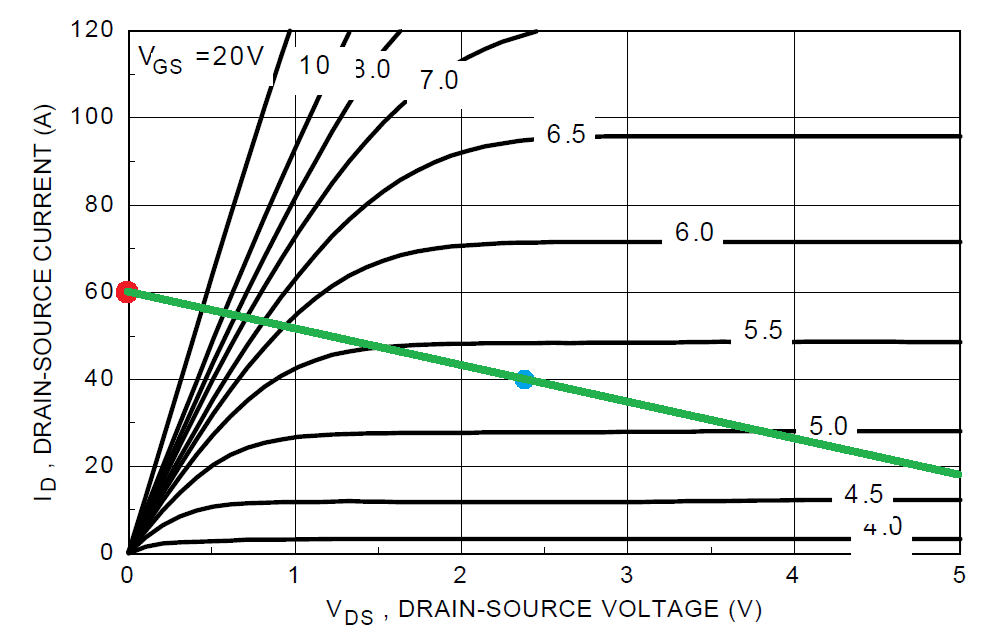
\includegraphics[scale=0.33]{images-worksheet2-solutions/loadline}
\\}

Looking at the $I_D$ vs. $V_{DS}$ curve for $V_{GS}=5.5V$, the intersection is at around $V_{DS}=1.5, I_D=50A$. Using the same strategy as above, we have $P=I^2 \times R_{MOT}=(50A)^2 \times 0.06\Omega=150W$ from the motor and $P=V_{DS} \times I=1.5V \times 50A=75W$ from the MOSFET.

\section{Problem 4}

The intersection for $V_GS=20V$ is at around $V_{DS}=0.5, I_D=54A$. Using the same strategy as above, we have $P=I^2 \times R_{MOT}=(55A)^2 \times 0.06\Omega=181.5W$ from the motor and $P=V_{DS} \times I=0.5V \times 55A=27.5W$ from the MOSFET.

\end{document}

